\documentclass{article}
\usepackage{amsmath,amssymb,graphicx,tikz}
\usepackage{hyperref}
\usepackage{tikz}
\usepackage{amsfonts}
\usepackage{amsmath}
\usepackage{listings}
\usepackage{pgfplots}
\usepgfplotslibrary{statistics}

\title{STA248 Winter 2016, Assignment 1}
\author{Connor Peet \#1001088208}
\renewcommand{\today}{~}
\hypersetup{pdfpagemode=Fullscreen,
  colorlinks=true,
  linkfileprefix={}}
\begin{document}
\maketitle

\lstset{
    numbers=left
}

\begin{enumerate}
\item [1.]
    \begin{enumerate}
    \item [(a)] $p_{60/100} = 11$
    \item [(b)] $p_{30/100} = 8$
    \item [(c)] When we're looking for percentiles, we're looking for the `closest' $y$ where $\int^y_z cdf(x) \leq \texttt{Percentile}$. The percentiles of discrete distributions is somewhat approximate; because there are a finite number of values a parameter may take on, the \textit{n}th percentile may appear slightly more often than expected. \\
    However, continuous functions can take on any value in the domain, so the first fundamental theorem of calculus guarantees that we will be able to find an exact value of $y$ such that $\int^y_z cdf(x) = \texttt{Percentile}$. Therefore, for continuous random variables, $P[X \leq p_{k / 100}] = k / 100$.
    \item [(d)] From the textbook, the density function of the exponential distribution is defined as $\frac{1}{\beta} e^{-x / \beta}$.
        \begin{equation*}
        \begin{aligned}
        \int_0^p \frac{1}{1} e^{-x / 1} &= 0.2 \\
        \int_0^p e^{-x} &= 0.2 \\
        (-e^{-p}) - (-e^{-0}) &= 0.2 \\
        e^{-p} &= 0.8 \\
        p &= - \ln 0.8
        \end{aligned}
        \end{equation*}
    \end{enumerate}
\item [2.]
    \begin{enumerate}
    \item [(a)] The data appears to form an exponential distribution.
        \begin{center}
        \begin{tabular}{ r | l }
            9  & 105130611002 \\
            10 & 1507 \\
            11 & 4106 \\
            12 & 02 \\
            13 & 13
        \end{tabular}
        \end{center}
    \item [(b)] The mean value of the sample is $\bar{X} = 10.2917$ thousand hours.
    \item [(c)] The median lifespan is is $9.8$ thousand hours. This means that about half the bulbs failed sooner than this, and half failed later. Taking a random bulb, you can expect it to last about $9.8$ thousand hours.
    \item [(d)] The variance $\sigma^2 = 1.8938$ and the standard deviation is $\sigma = 1.3762$.
    \item [(e)] The provided statement is based on the \textit{normal} probability rule, but an exponential distribution is far from normal. The statement is therefore not necessarily correct; in our own small sample, for instance, over eight percent of values fell outside that range.
    \item [(f)] Chebyshev's inequality says that $\forall k \in \mathbb{R}^+, P(|X - \mu | < k \sigma) \geq 1 - \frac{1}{k^2}$. To chose a $k$, calculate $13.050 - 10.2817 \approx 10.2817 - 7.530 \approx 2.7627 = k\sigma$, so $k = 2.007$. We can then plug in the rest of the values found previously to discover $P(|X - 10.2917 | < 2.7627) \geq 1 - \frac{1}{2.007^2}$. Therefore, we can estimate $P(7530 < X < 13050) = 0.7519$.
    \end{enumerate}
\item [3.]
    \begin{enumerate}
    \item [(a)]
        \begin{equation*}
        \begin{aligned}
        f(x) &= (1 + \theta)x^\theta \\
        f(x) &= x^\theta + \theta x^\theta \\
        \int_{0}^1 f(x) dx &= \int_{0}^1 (x^\theta + \theta x^\theta) dx \\[10pt]
        H(x) &= \frac{1}{\theta + 1}x^{\theta + 1} + \frac{\theta}{\theta + 1} x^{\theta + 1} \\
             &= \frac{\theta + 1}{\theta + 1}x^{\theta + 1} = x^{\theta + 1} \\[10pt]
        \int_{0}^1 f(x) dx &= H(1) - H(0) \\
                           &= 1^{\theta + 1} - 0^{\theta + 1} = 1
        \end{aligned}
        \end{equation*}
    \item [(b)]
        \begin{equation*}
        \begin{aligned}
        E[X] &= \int_0^1 xf(x) dx \\
        &= \int_0^1 (1 + \theta)x^{\theta + 1} dx \\
        &= \frac{\theta + 1}{\theta + 2}
        \end{aligned}
        \end{equation*}
    \item [(c)]
        \begin{equation*}
        \begin{aligned}
        \mu &= \frac{\theta + 1}{\theta + 2} \\
        \mu\theta + 2\mu &= \theta + 1 \\
        \mu\theta - \theta &= -2\mu + 1 \\
        \theta &= \frac{-2\mu + 1}{\mu - 1}
        \end{aligned}
        \end{equation*}
    \item [(d)]
        \begin{equation*}
        \begin{aligned}
        \bar{X} &= \frac{0.5 + 0.3 + 0.1 + 0.1 + 0.2}{5} = 0.24 \\
        \hat{\theta} &= \frac{-2 \times 0.24 + 1}{0.24 - 1} \approx -0.6842
        \end{aligned}
        \end{equation*}
    \end{enumerate}
\item [4.]
    \begin{enumerate}
    \item [(a)] See below:
        \begin{figure}[h]
        \begin{center}
        \begin{tabular}{ r | l }
        6 & 4 \\
        6 & 89 \\
        7 & 01234 \\
        7 & 555678889 \\
        8 & 01344 \\
        8 & 55 \\
        9 &  \\
        9 & 9
        \end{tabular}
        \end{center}
        \end{figure}
    \item [(b)] The outlier is the $9.9$ data point. See the graph below:
        \begin{figure}[h]
        \centering
            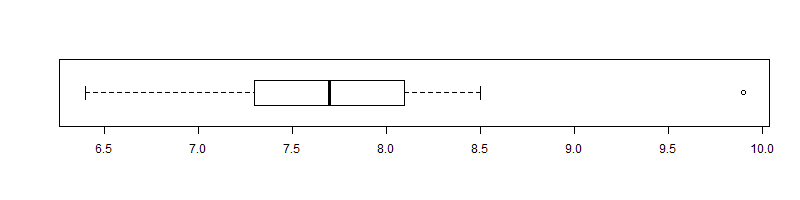
\includegraphics[width=\textwidth]{sta248-a1-q4}
        \end{figure}
    \item [(c)] The data point is a result of an experimental error, and is not an reflect an accurate measurement of the coating thickness. It should therefore be excluded from the study.
    \end{enumerate}
\item [5.]
    \begin{enumerate}
    \item [(a)] The distribution looks similar to a normal distribution with a mean at or slightly lower than $4$. Eyeballing it, I'd estimate the standard deviation of that distribution a bit under $2$.
        \begin{figure}[h]
        \centering
            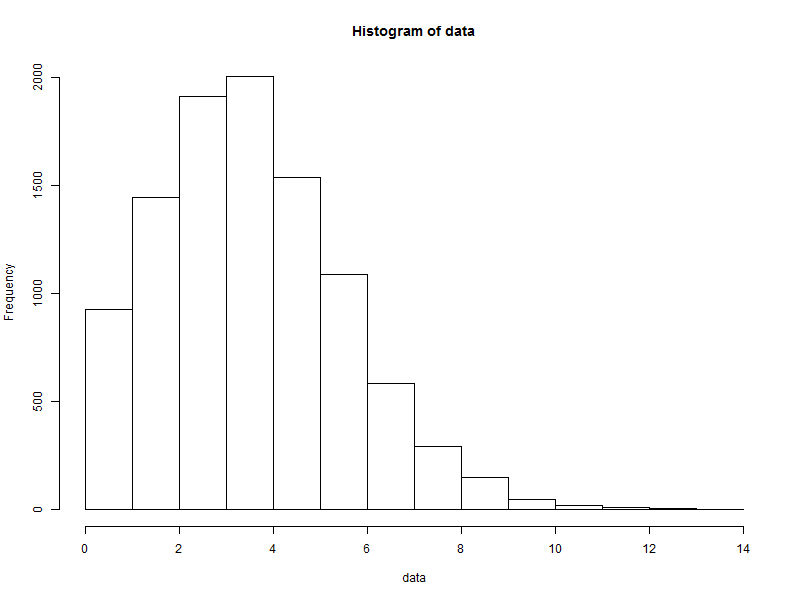
\includegraphics[width=\textwidth]{sta248-a1-q5-a}
        \end{figure}
    \item [(b)] In R, I called \texttt{mean(rpois(16, 4))}, which gave the unsurprising output of $4.0625$.
    \item [(c)]
        \begin{enumerate}
        \item See below for the histogram.
        \begin{figure}[h]
        \centering
            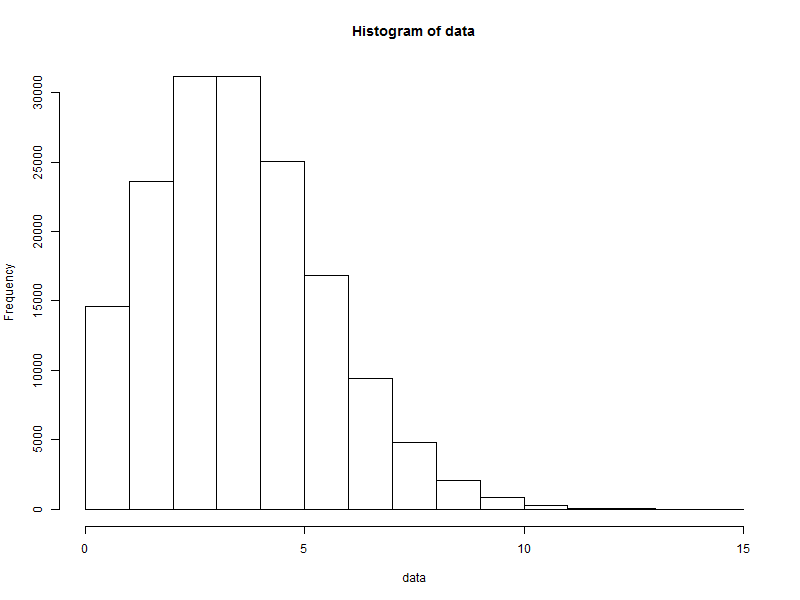
\includegraphics[width=\textwidth]{sta248-a1-q5-c}
        \end{figure}
        \item Mean: $4.0015$.
        \item Standard deviation: $1.9997$.
        \item This is about what I expected. In previous classes, we learned that large samples of the Poisson distribution are exceptionally well-represented by a normal distribution with a mean of $\lambda$ and a variance of $\sigma = \sqrt{\lambda}$, and additionally the central limit theorem indicates that this would occur.
        \end{enumerate}
    \item [(d)] For larger samples, I would expect the values in the previous parts to be even closer to the expected values of $4$ and $2$. When running a simulation in R with this larger sample size, the mean is $4.0002$ and the standard deviation is $2.001$, which are indeed closer to the expected values.
    \end{enumerate}
\end{enumerate}

\newpage
\appendix
\section{Code for Question 5A}
\lstinputlisting[language=R]{sta248-a1-q5-a.r}
\section{Code for Question 5C}
\lstinputlisting[language=R]{sta248-a1-q5-c.r}
\end{document}
